\documentclass[11pt,letterpaper]{article}
\usepackage[margin=1in]{geometry}
\usepackage[utf8]{inputenc}
\usepackage[T1]{fontenc}
\usepackage{hyperref}
\renewcommand{\familydefault}{\sfdefault}
\usepackage{helvet}
\pagestyle{empty}
\usepackage[kerning=true]{microtype}
\usepackage{parskip}
\usepackage{sansmath}
\usepackage{graphicx}
\usepackage{sidecap}  
\sidecaptionvpos{figure}{c}
\usepackage{float}
\usepackage{color, soul}
% Feel free to use additional packages for glosses, figures, whatnot.
\usepackage[dvipsnames]{xcolor}
\newcommand{\mf}[1]{\textcolor{BurntOrange}{[MF: #1]}}
\newcommand{\pt}[1]{\textcolor{Cerulean}{[PT: #1]}}
\newcommand{\bvt}[1]{\textcolor{ForestGreen}{[BvT: #1]}}
% The next bit is for reserving sufficient space for authors,
% affiliations, and e-mail address.  No need to change for initial
% anonymous version.  For the final version, replace the
%\toggletrue{anonymous} %with \togglefalse{anonymous} to de-anonymize.
\usepackage{etoolbox}
\newtoggle{anonymous}
\toggletrue{anonymous}

\renewcommand{\title}[1]{\textbf{#1}\\}
\newcommand{\authors}[1]{\iftoggle{anonymous}{\phantom{#1}}{#1}\\}
\newcommand{\email}[1]{\iftoggle{anonymous}{\phantom{#1}}{#1}}

\begin{document}

% First page:

% Insert title, authors, affiliations, and e-mail address in the next three lines:

\title{The role of relevance, competence and priors for scalar implicatures}
\authors{Michael Franke (University of T\"ubingen), Bob van Tiel (Radboud University), Polina Tsvilodub (Osnabr\"uck university)}
\email{pstvilodub@uos.de}

% Here goes the main text of your abstract:

If someone says "Anna ate some cookies." the hearer of this sentence might infer the upper-bounded reading that Anna ate \textit{some, but not all} cookies. Similarly, given the sentence "Donald ate a donut or a pretzel." one might infer an exclusive interpretation, i.e., that Donald ate either \textit{the donut or the pretzel, but not both}. 
Both inferences are considered as instances of \textit{scalar implicature (SI)}---an inference based on the comparison to a salient informationally stronger alternative ``all'' or ``and'', respectively [2,3]. That is, the listener might arrive at these interpretations by reasoning about the epistemic state of a cooperative rational speaker [4]. %: if the stronger alternative was true, a rational agent would have used the stronger utterance; but since she did not, she must have lacked the evidence for using ``all'' 
%(Grice, 1975).
%Some prior work addresses the influence of sentence structure, or of specific linguistic markers on the robustness of SIs (Li, 2021). Moreover, 
Literature suggests that, among others, three factors influence the robustness of scalar implicatures: (1) \textit{relevance} of the stronger alternative to the listener, (2) the \textit{competence} of the speaker about the truth of the stronger alternative, and (3) the \textit{prior probability that the stronger alternative is true} [1,3,5]. However, their influence was mostly investigated in isolation in prior work. We aim to fill this gap by exploring how these three factors influence the robustness of scalar implicatures in combination, when the SI triggers ``some'' and ``or'' are presented in rich context. Simultanously, we directly compare whether the two triggers are both influenced by these factors as predicted by the SI account.

In our web-based rating study (LINK), participants read background stories which were designed to score either high or low with respect to each factor of interest (high/low prior probability of the more informative alternative $\times$ high/low speaker competence $\times$ high/low contextual relevance of the alternative $\times$ triggers), manipulated within-subjects. 
On critical trials, participants were asked to rate four sentences on a scale ranging from ``certainly true'' to ``certainly false'' (converted to 0--100), one per factor and one containing an upper-bounded (or exclusive) paraphrase of the trigger. The sentences elicited judgements of how likely it is that each factor was high, and how likely the critical scalar implicature was true (s. transcript). If the SI account is true, on average, we expect higher likelihood ratings for the scalar implicature statement, if the relevance and comptenece of the item were judged as high and the prior of the stronger alternative as low. Each participant saw eight stories (four per trigger) sampled from 32 stories per trigger, randomly shuffled with eight visually identical attention checks and comprehension questions.

%(71  excluded following preregistered exclusion criteria).
We analysed data from 206 participants recruited through Prolific; their ratings were z-scored within each factor by-participant. We analysed the results using a Bayesian linear mixed effects model, regressing the implicature likelihood rating against the fixed effects of all factor ratings by the same participant for that vignette, the effect of trigger, all interactions and maximal tractable random effects structure. Participants' factor ratings agreed well with the prior classification of the items (Fig.~\ref{by-item-ratings}, colors).
%Consistent with predictions of the SI account, for the trigger ``some'', we find a clear negative prior probabilty effect of the stronger alternative ``all'' being true (probability of the effect of prior being smaller than 0.05: $P = 0.999$). 
As predicted by the SI account, participants are more likely to infer the ``some, but not al'' reading when they judged the prior probability of ``all'' being true as low ($P=0.999$ for the effect being $<0.05$, Fig.\ref{posteriors} for all results). They also robustly infer the upper-bounded interpretation when judging speaker competence as high ($P=1$ for effect $>0.05$).
%Similarly, we find a clear positive effect for speaker competence (effect larger than 0.05 probability: $P =  1$). We do not find any clear effects of relevance. 
However, participants were only more likely to infer the ``A or B, but not both'' reading when they rated the speaker competence as high  ($P=0.993$ for effect $>0.05$). No relevance effects were found for both triggers.
%For the trigger ``or'', we only find a positive effect of competence ($P =  0.993$). 
Further, we computed exploratory pairwise correlations of all the predictors. While no correlations were found for ``some'', we find a significant correlation between the prior and the relevance effects for ``or'' ($R^2 = -0.106, p=...$), and a significant correlation between competence and relevance ($R^2 = 0.127, p=...$) for ``or''. This suggests that these factors might be interdependent in case of ``or''.
Overall, our results support the SI account, but also indicate that these factors might have a more fine-grained influence on the robustness of SI generation in combination.%, especially for disjunction interpretation.
%Overall, the results provide moderate evidence for the scalar implicature account of ``some'' and ``or'', but also indicate that there might be intricate dependencies between the factors' influence on the robustness of SI, especially for disjunction interpretation.
\newpage

% Second page for additional materials, example stimuli, graphs, tables, references:


\begin{figure}
   \makebox[\linewidth][c]{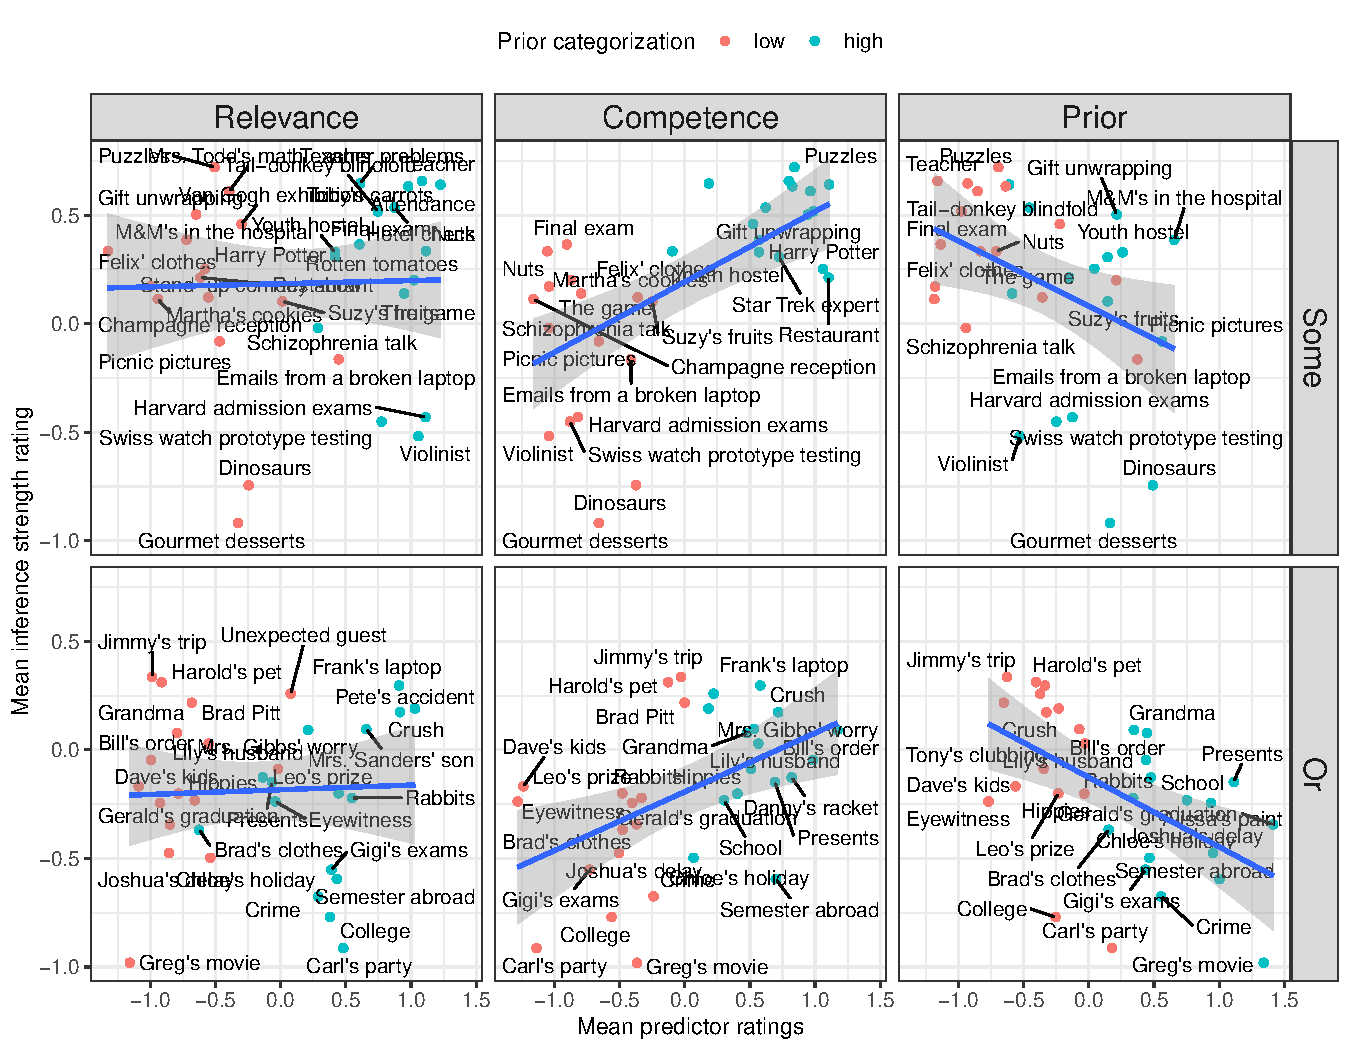
\includegraphics[width=0.7\linewidth]{byItem-ratings.pdf}}%
 \caption{Relating ratings for relevance, competence and prior statements (x-axis) to
ratings for the strength of pragmatic enrichments (y-axis). The top row shows ratings,
averaged for each story for ``some'' (enriched to ``some, but not all''). The bottom row shows ratings, averaged for each story for ``or'' (enriched to ``A or B, but not both'').}
    \label{by-item-ratings}
\end{figure}

\begin{figure}   
    \makebox[\linewidth][c]{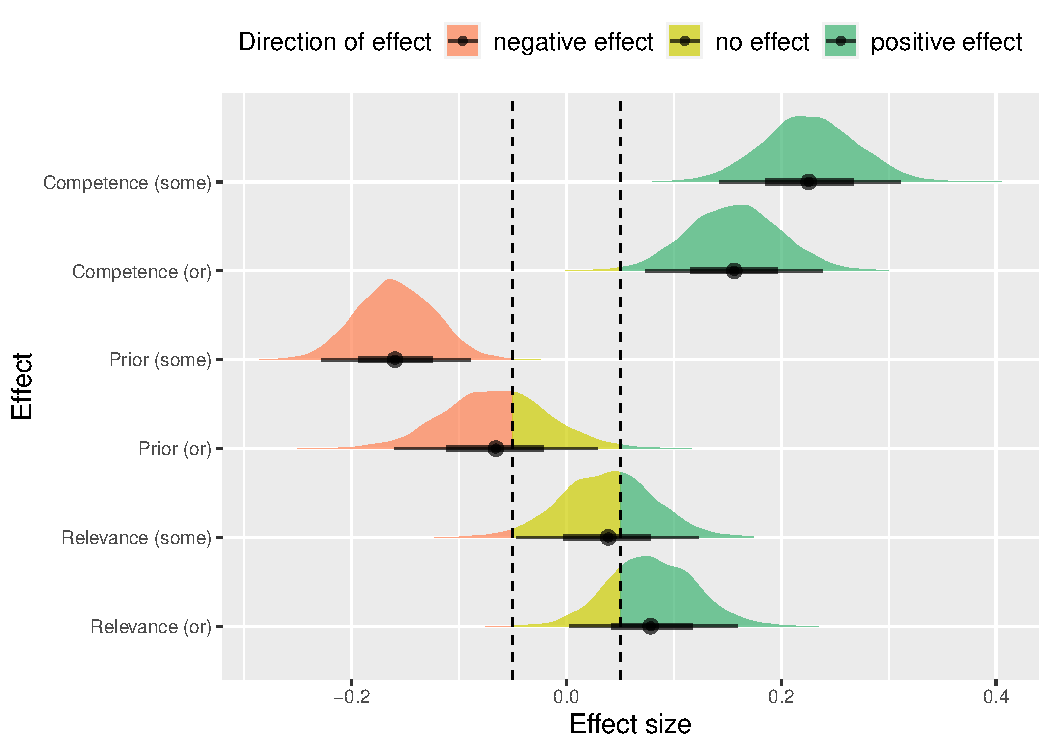
\includegraphics[scale=0.7]{posterior-effects.pdf}}
    \caption{Distributions of posterior samples for the effects of each predictor for each trigger (y-axis). The colors indicate the fraction of the distribution density corresponding to a positive, no or a negative effect. \newline \textbf{References:} [1] Degen, J., Tessler, M. H., \& Goodman, N. D., In \textit{Proceedings of CogSci}, 2015 [2] Geurts, B., \textit{Quantity Implicatures}, 2010 [3] Goodman, N. D., \& Stuhlm\"uller, A., In \textit{Topics in Cognitive Science}, 5(1), 2013 [4] Grice, H. P. In \textit{Syntax and semantics, vol. 3: Speech acts}, 1975 [3] Horn, L. R., 1972 [5] Sperber, D., \& Wilson, D., \textit{Relevance: communication and cognition}, 1995  
    }
    \label{posteriors}
\end{figure}

%\begin{SCfigure}[1.7]
%    \includegraphics[ scale=0.5]{amlap_expt4_double_mod2.pdf}
 %   \caption{Pilot Results: Inferred basic-level comparison classes (e.g. ‘...big relative to other \textit{dogs}’) when the directly modified subordinate N (‘big Great Dane’) appears in different syntactic positions (x-axis).\newline
%    \newline \textbf{References:} [1] Kamp, J., In \textit{Formal semantics of natural language}, 1975  [2] Kennedy, C., \textit{Linguistics and Philosophy, 30(1)}, 2007 [3] Tessler, M. H.; Lopez-Brau, M.; Goodman N. D., In \textit{39th annual meeting of the Cognitive Science society}, 2017
%    \label{double-mod}[4] Reboul, A., In \textit{Language typology and language universals, an international handbook, vol.1}, 2001}
%\end{SCfigure}

\newpage

% Optional third page for additional information if the investigated language is not English:
\end{document}
